\section{Matrix representation of WFSA}

\subsection{Simple WFSA}

We consider the set of WFSA $\mathbb{A}$ that has a unique initial state (denoted $0$ by convention), has at most one transition between two states, no $\epsilon$ transition and all the arcs going to the same state share the same label, i.e. $\forall e_1, e_2 \in E$, $n[e_1] = n[e_2] \implies \lambda[e_1] = \lambda[e_2]$. By definition, any automaton $\mathcal{A} \in \mathbb{A}$ can be represented as a simple directed graph --- a graph with at most one edge between two vertices. For this reason, we denote such automaton a \emph{simple WFSA}. Remark that simple WFSA are as expressive as standard WFSA since any WFSA can be transformed to an equivalent simple WFSA \textcolor{red}{[PROOF: algorithm / process to convert a general WFSA to a simple WFSA]}. Fig. \ref{fig:wfsa} shows an example of WFSA and an equivalent simple WFSA. 
%
\begin{figure}[t] % ’ht’ tells LaTeX to place the figure ’here’ or at the top of the page
    \centering 
    \subcaptionbox{common WFSA.}
        {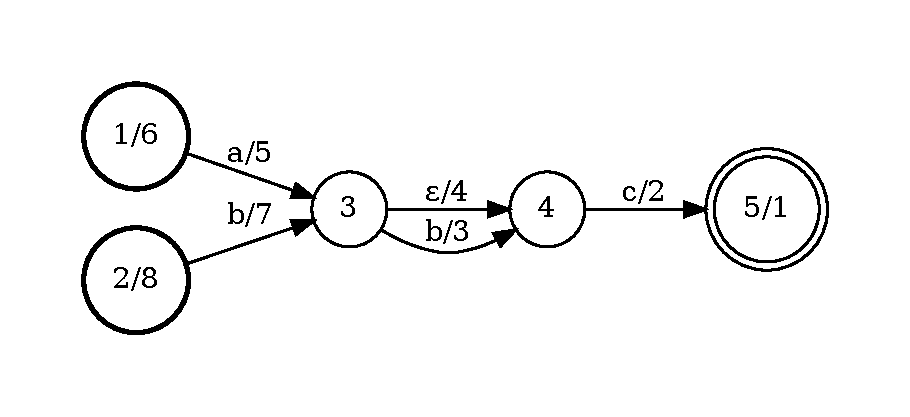
\includegraphics[width=0.7\linewidth]{images/reg_fsa.pdf}}
    \subcaptionbox{\label{simple} simple WFSA.}
        {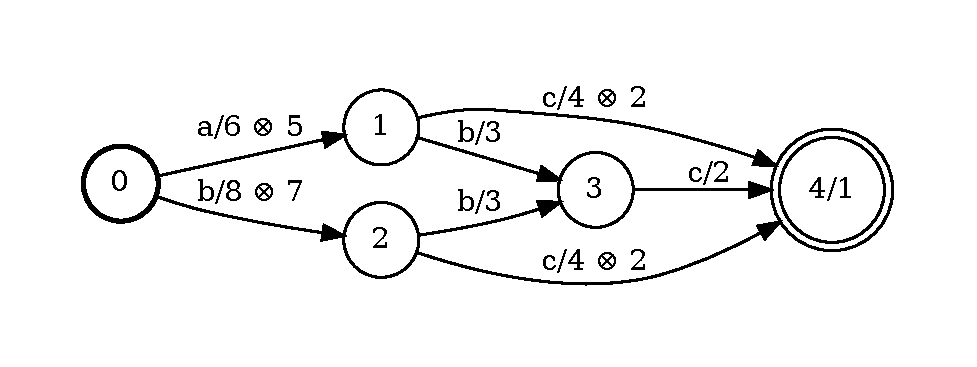
\includegraphics[width=0.7\linewidth]{images/simple_fsa.pdf}}
    \caption{Example of equivalent WFSA accepting the sequences $abc, ac, bbc$, and $bc$.}
    \label{fig:wfsa}
\end{figure}
%

\subsection{Representing simple WFSA in a K-vector space}
\paragraph{} The advantage of simple WFSA is that they can be represented by matrix and vector allowing a linear algebraic treatment of WFSA. Let's consider a simple WFSA $\mathcal{A} = (\Lambda, Q, \{0\}, F, \alpha, \omega, E)$, $\mathcal{A} \in \mathbb{A}$, over the semiring $K = (\mathbb{K}, \oplus, \otimes, \bar{0}, \bar{1})$. We denote $Q' = Q \setminus \{0\}$ the set of states in $\mathcal{A}$ not including the initial state $0$. Let be $S = (\mathbb{K}^{|Q'|}, +, \cdot)$ a $K$-vector space and let be $B$ the standard basis of $S$
\begin{align}
    \mathbf{B} &= \{ \begin{bmatrix} b_{q,1}, \dots, b_{q,|Q'|} \end{bmatrix}^\top : b_{q,i} = \begin{cases} \bar{1} & \text{if $i = q$} \\ \bar{0} & \text{otherwise} \end{cases}\text{, } \forall q \in Q' \}.
\end{align}
The automaton $\mathcal{A}$ can be encoded in terms of an initial weight $K$-vector
\begin{align}
    \boldsymbol{\alpha} &= \sum_{q \in \{e : p[e] = 0, \forall e \in E\}} \alpha(q) \mathbf{b}_{q}, 
\end{align}
a transition $K$-matrix 
\begin{align}
    \mathbf{T} = \sum_{e \in E} w[e] \mathbf{b}_{p[e]} \mathbf{b}_{n[e]}^\top,
\end{align}
a final $K$-vector 
\begin{align}
    \boldsymbol{\omega} &= \sum_{q \in F} \omega(q) \mathbf{b}_{q},
\end{align}
and a vector of label $\boldsymbol{\lambda} \in \Lambda^{|Q'|}$ where $\lambda_q$ is the label associated to the state $q$. The special case of accepting the emtpy string $\epsilon$ is encoded as an extra parameter
\begin{align}
    \rho = \begin{cases}
     \alpha(0) \otimes \omega(0) & \text{if $0 \in F$} \\
     \bar{0} & \text{otherwise}
    \end{cases}.
\end{align}
Hereafter, for a simple WFSA $\mathcal{A}$, we slightly abuse the notation and we write $\mathcal{A} = (\Lambda, Q, \{0\}, F, \alpha, \omega, E)$ or $\mathcal{A} = (\Lambda, Q, \boldsymbol{\alpha}, \mathbf{T}, \boldsymbol{\omega}, \rho, \boldsymbol{\lambda})$ interchangeably.

\subsection{Kernel and Cokernel of $\mathbf{T}$}

We say a state $q \in Q \setminus \{0\} $ is a root state if there is no transition leaving a state in $Q \setminus \{0\}$ and reaching $q$. Stated algebraically, $q$ being a root state implies
\begin{align}
    \forall i \in Q \setminus \{0\}, \;\mathbf{b}_i^\top \mathbf{T} \mathbf{b}_q = \mathbf{0} \implies \mathbf{T} \mathbf{b}_q = \mathbf{0}.
\end{align}
Consequently, the subspace defined the subset of basis associated to the subset of root states of $\mathcal{A}$ is given by the kernel of $\mathbf{T}$, $\text{ker}(\mathbf{T}) = \{ \mathbf{x} : \mathbf{T} \mathbf{x} = \mathbf{0},\; \forall x \in \mathbb{S}\}$. 

\paragraph{} We say a state $q \in Q \setminus \{0\} $ is a leaf state if there is no transition leaving $q$
\begin{align}
    \forall i \in Q \setminus \{0\}, \;\mathbf{b}_q^\top \mathbf{T} \mathbf{b}_i = \mathbf{0} \implies \mathbf{b}_q^\top \mathbf{T} = \mathbf{0}^\top.
\end{align}
Consequently, the subspace defined the subset of basis associated to the subset of leaf states of $\mathcal{A}$ is given by the cokernel of $\mathbf{T}$, $\text{ker}(\mathbf{T}^\top) = \{ \mathbf{x} : \mathbf{x}^\top \mathbf{T} = \mathbf{0}^\top,\; \forall x \in \mathbb{S}\}$. 

\subsection{Evaluating $W(\mathcal{A})$}

Representation of a simple WFSA $\mathcal{A}$ in terms of a K-matrix naturally leads to an easy and efficient way of calculating the sum $W(\mathcal{A})$. Let be $\boldsymbol{\pi}$ an accepted path of length $n$. The weight of a transition $e_i$ from $q_1$ to $q_2$ is given by
\begin{equation}
    w[e_i] = \mathbf{b}_{q_1}^\top \mathbf{T} \mathbf{b}_{q_2}. 
\end{equation}
The $\oplus$-sum of all path of length $2$ leaving $q_1$ and ending in $q_2$ is given by:
\begin{align}
    \Pi_2(\{q_1\}, \{q_2\}) &= \bigoplus_{i \in Q \setminus \{0\}} (\mathbf{b}_{q_1}^\top \mathbf{T} \mathbf{b}_{i}) \otimes (\mathbf{b}_{i}^\top \mathbf{T} \mathbf{b}_{q_2}) \\
    &= \mathbf{b}_{q_1}^\top \mathbf{T} \bigg( \sum_{i \in Q \setminus \{0\}} \mathbf{b}_{i} \mathbf{b}_{i}^\top \bigg) \mathbf{T} \mathbf{b}_{q_2} \\
    &= \mathbf{b}_{q_1}^\top \mathbf{T} \mathbf{T} \mathbf{b}_{q_2}. \label{eq:sum_l2}
\end{align}
Eq. \eqref{eq:sum_l2} can be extended to an arbitrary path length $k$ and arbitrary set of starting states $A \subseteq Q \setminus \{0\}$ and ending states $B \subseteq Q \setminus \{0\}$
\begin{align}
    \Pi_n(A, B) &= \bar{\mathbf{b}}_A^\top  \mathbf{T}^n \bar{\mathbf{b}}_B \label{eq:sum_paths}
\end{align}
where $\bar{\mathbf{b}}_A = \sum_{q \in A} \mathbf{b}_q$, $\bar{\mathbf{b}}_B = \sum_{q \in B} \mathbf{b}_q$ and 
\begin{equation} 
    \mathbf{T}^n = \underbrace{\mathbf{T} \dots \mathbf{T}}_{n \text{ times}}.
\end{equation}
is the $k$th power of the $K$-matrix $\mathbf{T}$. With \eqref{eq:sum_paths} and taking into account the initial and final weights $\boldsymbol{\alpha}$ and $\boldsymbol{\omega}$, one can express $W(\mathcal{A})$ as the $\oplus$-sum of all the path of length 0, 1, 2, ...
\begin{align}
    W(\mathcal{A}) &= \rho \oplus \bigoplus_{n=1}^\infty \boldsymbol{\alpha}^\top \mathbf{T}^n \boldsymbol{\omega}. \label{eq:total_sum}.
\end{align}

\begin{align}
    W(\mathcal{A}) &= \rho \oplus \boldsymbol{\alpha}^\top ( \mathbf{T}^0 + \mathbf{T}^1 + \mathbf{T}^2 + ...   )\boldsymbol{\omega} \label{eq:total_sum}
\end{align}

\begin{align}
    \mathbf{T}_C &= \mathbf{M}^\top (\mathbf{T}_A \otimes \mathbf{T}_B) \mathbf{M}
\end{align}


\paragraph{} Eq. \eqref{eq:total_sum} naturally lends itself to a recursive computation: 
\begin{align}
    \mathbf{u}_1 &= \boldsymbol{\alpha} \\
    \mathbf{u}_n &= (\mathbf{u}_{n-1}^\top \mathbf{T})^\top \label{eq:forward_rec}
\end{align}
leading to 
\begin{align}
    W(\mathcal{A}) &= \rho \oplus \bigoplus_{n=1}^\infty \mathbf{u}_n^\top \boldsymbol{\omega}.
\end{align}

\paragraph{} Eq. \eqref{eq:forward_rec} leads to an interesting observation: a simple WFSA can be interpreted as linear dynamical system in a $K$-vector space representing the states of the automaton. The recursion to evaluate of the automaton's weight $W(\mathcal{A})$ is analog to evaluate a trajectory from the initial configuration $\boldsymbol{\alpha}$. An illustration is given in Fig. \ref{fig:ldyn_wfsa}.
%
\begin{figure}[t] 
    \centering 
    \subcaptionbox{simple WFSA $\mathcal{A}$ with initial weights parameterized by $\sigma$.}
        {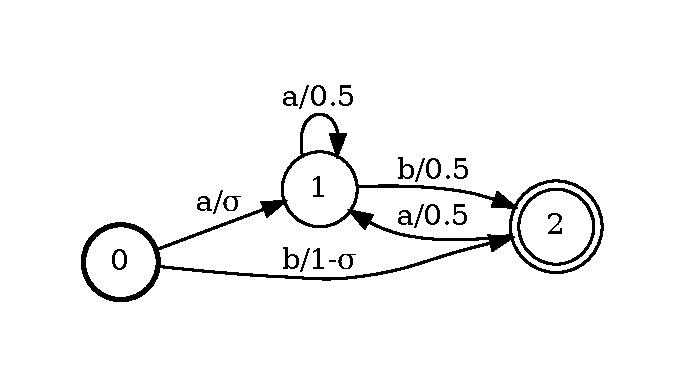
\includegraphics[width=0.49\linewidth]{images/swfsa.pdf}}
    \subcaptionbox{\label{simple} $K$-vector space representing the state-space of $\mathcal{A}$.}
        {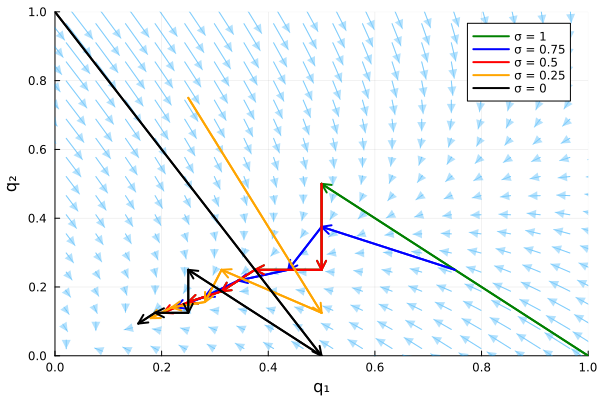
\includegraphics[width=0.49\linewidth]{images/dyn_system.png}}
    \caption{Visualisation of trajectories as a function of $\sigma$ taken while computing $W(\mathcal{A})$. The blue arrows in background represent the linear dynamical system induced by the transition matrix}
    \label{fig:ldyn_wfsa}
\end{figure}

\subsection{Acyclic Simple WFSA}

By definition, an acyclic simple WFSA $\mathcal{A}$ can only accept path whose length are less than $|Q \setminus \{0\}|$. This implies that there exists a $k \leq |Q \setminus \{0\}| + 1$ such that 
\begin{align}
    \forall \boldsymbol{\alpha}, \boldsymbol{\omega} \in \mathbb{S}^{|Q \setminus \{0\}|} \; \boldsymbol{\alpha}^\top \mathbf{T}^k \boldsymbol{\omega} = \bar{0}.
\end{align}
Consequently, the transition matrix of $\mathcal{A}$ is nilpotent, i.e. $\mathbf{T}^k = \mathbf{0}$ for some $k$.

\paragraph{} The consequence of this result is that, as one would expect, the $\oplus$-sum in \eqref{eq:total_sum} is finite for acyclic simple WFSA
\begin{align}
    W(\mathcal{A}) &= \rho \oplus \bigoplus_{n=1}^{\max_{\boldsymbol{\pi}} |\boldsymbol{\pi}|} \boldsymbol{\alpha}^\top \mathbf{T}^n \boldsymbol{\omega}.
\end{align}
It allows therefore to define a another recursion going backward 
\begin{align}
    \mathbf{v}_n &= \boldsymbol{\omega} \\
    \mathbf{v}_n &= \mathbf{T} \mathbf{v}_{n+1} \\
    W_n(\mathcal{A}) &= \rho \oplus \boldsymbol{\alpha}^\top \mathbf{v}_n.
    \label{eq:sum_paths_rec_swfsa_b}
\end{align}
Finally both recursions can be combined, for $1 < m < n$ we have
\begin{equation}
    W_n(\mathcal{A}) = \rho \oplus \mathbf{u}_m^\top 
    \mathbf{v}_{m+1}.
\end{equation}
 
%  We define its simple graph representation $L(\mathcal{A})$   
% constructed in the following way:
% \begin{enumerate}
%     \item for every edge $e \in E$ make a new labeled state in $L(\mathcal{A})$ with label $\lambda[e]$;
%     \item for every edge $e \in E$ we assign an initial weight $\alpha(p[e]) \otimes w[e]$ and a final weight $\omega(n[e])$ to the corresponding vertex in $L(\mathcal{A})$; 
%     \item for every two edges $e_1, e_2 \in E$ such that $n[e_1] = p[e_2]$ make a directed edge in $L(\mathcal{A})$ with weight $w[e_2]$ between their corresponding vertices;
%     \item for every pair of edge $e_1, e_2$ in $L(\mathcal{A})$ connected head-to-tail in a vertex with label $\epsilon$ add a new edge from $p[e_1]$ to $p[e_2]$ with weight $w[e_1] \otimes w[e_2]$;
%     \item for every vertex $v$ in $L(\mathcal{A})$ with label $\epsilon$, remove $v$ from $L(\mathcal{A})$  and for every pair of edge $e_1, e_2$ connected head-to-tail in $v$ add a new edge from with weight $w[e_1] \otimes w[e_2]$. 
% \end{enumerate}
% An illustration of $L(\mathcal{A})$ where $\mathcal{A}$ is defined as in Fig. \ref{fig:standard_fsa} is shown in Fig. \ref{fig:simplegraph_wfsa}.
%

\subsection{Weighted Pushdown Automata}

\begin{align}
    \mathbf{v}_n^{(1)} &= \mathbf{T}^{(1) \top} \mathbf{v}_{n-1}^{(1)} + \mathbf{\bar{P}}^{(2)} \mathbf{u}_{n-1}^{(2)} \\
    \vdots \\
    \mathbf{v}_n^{(i)} &= \big( \mathbf{1}_{N^{(i-1)}} \otimes \mathbf{T}^{(i) \top} \big) \mathbf{v}_{n-1}^{(i)} + \mathbf{P}^{(i-1)} \mathbf{w}_{n-1}^{(i-1)}  + \mathbf{\bar{P}}^{(i+1)} \mathbf{u}_{n-1}^{(i+1)}  \\
    \vdots \\
    \mathbf{v}_n^{(d)} &= \big( \mathbf{1}_{N^{(d-1)}} \otimes \mathbf{T}^{(d) \top} \big) \mathbf{v}_{n-1}^{(d)} + \mathbf{P}^{(d-1)} \mathbf{w}_{n-1}^{(d-1)} 
\end{align}


\begin{align}
    \mathbf{w}_n^{(1)} &= \mathbf{v}^{(1)}_n \\
    \mathbf{w}_n^{(i)} &= \mathbf{P}^{(i-1)} \mathbf{w}_{n}^{(i-1)}  \\
    \mathbf{u}_n^{(d)} &= \mathbf{u}^{(d)}_n \\
    \mathbf{u}_n^{(i)} &= \mathbf{\bar{P}}^{(i+1)} \mathbf{u}_{n}^{(di+1)}
\end{align}
